\section{Methodology}
This section outlines the implementation pipeline developed for replicating and extending the referenced fraud detection framework. We begin by preprocessing the dataset and training an autoencoder exclusively on fraudulent transactions to learn their underlying distribution. This autoencoder is then used to generate synthetic fraudulent samples, which are subsequently filtered using a Support Vector Machine (SVM) to ensure data quality. The resulting dataset is used to train an attention-based Long Short-Term Memory (ALSTM) network integrated into a gradient boosting ensemble for final classification. Each stage of the pipeline is detailed in the subsections that follow.

\subsection{Dataset Analysis and Preprocess}
The dataset employed in this project is the widely used \texttt{Credit Card Fraud Detection dataset}, made publicly available by \textit{Worldline and the Machine Learning Group at Université Libre de Bruxelles (ULB)}. The dataset is accessible for download from the \textit{Credit Card Fraud Detection}'s Kaggle repository\footnote{\url{https://www.kaggle.com/datasets/mlg-ulb/creditcardfraud}}.

This dataset contains transactions made by European cardholders over a period of two days in September 2013, comprising a total of 284,807 transactions, among which only 492 are labeled as fraudulent. This severe class imbalance (fraudulent transactions represent just 0.172\% of the total), as seen in Figure~\ref{fig:class-distribution}, makes it a challenging benchmark for anomaly detection and imbalanced classification tasks and motivates the use of specialized techniques such as synthetic data generation and class balancing strategies, which are detailed in subsequent sections.

Each transaction in the dataset is described by a total of 31 numerical features:
\begin{itemize}
    \item 28 features are anonymized principal components resulting from a \texttt{PCA} (Principal Component Analysis) transformation applied to the original dataset to preserve confidentiality (labeled from \texttt{V1} to \texttt{V28}).
    \item The remaining 3 features are:
        \begin{itemize}
            \item \texttt{Time}: The elapsed time (in seconds) from the first transaction in the dataset.
            \item \texttt{Amount}: The monetary amount of the transaction.
            \item \texttt{Class}: The target variable, where \texttt{1} indicates a fraudulent transaction and \texttt{0} indicates a legitimate one.
        \end{itemize}
\end{itemize}

\begin{figure}[h]
    \centering
    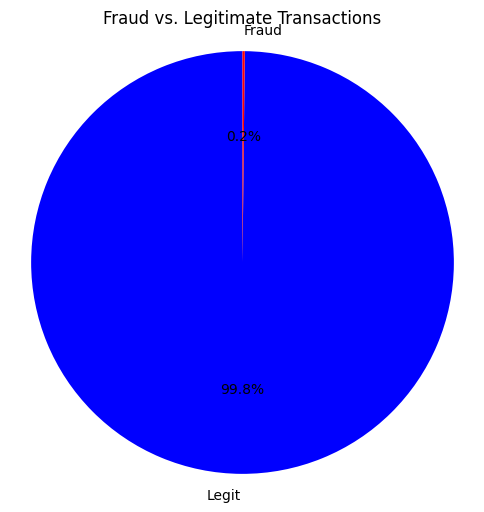
\includegraphics[width=0.25\textwidth]{images/fraud_vs_legit_pie.png}
    \caption{Distribution of Fraudulent vs. Legitimate Transactions}
    \label{fig:class-distribution}
\end{figure}

\subsubsection{Dataset Preprocess}
The dataset was preprocessed by removing the \texttt{Time} and \texttt{Label} columns. The \texttt{Time} feature was excluded based on recommendations from the original paper, as it did not significantly contribute to the learning process.

As suggested in the reference paper, the \texttt{Amount} feature was standardized using the \texttt{RobustScaler} transformation to reduce the influence of outliers, which are particularly common in financial transaction data.

\subsection{Autoencoder-based Fraud Pattern Modeling}
In our approach, we utilized an autoencoder neural network trained exclusively on fraudulent transactions to learn their internal structure and statistical properties. By exposing the model only to examples of fraud, we ensured its ability to specialize in recognizing the underlying data distribution of abnormal behaviors. This setup enables the model to generate new, synthetic fraud samples that maintain the intrinsic characteristics of real fraud cases.

To enhance the model’s generalization ability, we split the fraudulent samples into training and validation subsets. The reconstruction performance on the validation set guided model tuning and early stopping to prevent overfitting.

The autoencoder architecture is symmetric, with an encoder compressing the 29 input features through successive layers, and a decoder reconstructing the input by reversing the encoding path. Dropout regularization was employed in both parts of the network to combat overfitting by randomly deactivating a subset of neurons during training. Table~\ref{tab:autoencoder_architecture} summarizes the layer configuration of both encoder and decoder components.

The model was trained to minimize the reconstruction loss between the input $x$ and the output $\hat{x}$ using the Mean Squared Error (MSE) loss function:
\[
J(w, \hat{w}) = \frac{1}{n} \sum_{i=1}^{n} \frac{1}{2} \| x_i - \hat{x}_i \|^2
\]
Additionally, $L1$ regularization was applied to the network parameters to promote sparsity in the weights and reduce overfitting. The total loss function is a combination of MSE and the $L1$ norm:
\[
\mathcal{L}_{\text{total}} = \text{MSE} + \lambda \sum_{j} |w_j|
\]
where $\lambda$ is a regularization coefficient empirically set to $1 \times 10^{-3}$.

The model was trained using the \texttt{Adam} optimizer with an initial learning rate of $2 \times 10^{-4}$. A cosine annealing learning rate scheduler gradually reduced the learning rate over epochs, and early stopping was triggered if the validation loss did not improve for 75 consecutive epochs.

Once trained, the autoencoder was used to generate synthetic fraud samples by sampling latent representations and decoding them into realistic transaction vectors. These synthetic samples were later evaluated and filtered using a Support Vector Machine, as described in the following section.

\begin{table}[htbp]
    \small % or \scriptsize for even smaller
    \centering
    \begin{tabular}{|p{3.5cm}|p{3.5cm}|}
        \hline
        \textbf{Encoder} & \textbf{Decoder} \\
        \hline
        29 features (input) & 8 neurons, fully connected \\
        \hline
        23 neurons, fully connected & 17 neurons, fully connected \\
        \hline
        Dropout = 0.1 & Dropout = 0.2 \\
        \hline
        19 neurons, fully connected & 19 neurons, fully connected \\
        \hline
        Dropout = 0.2 & Dropout = 0.1 \\
        \hline
        17 neurons, fully connected & 23 neurons, fully connected \\
        \hline
        8 neurons, fully connected & 29 neurons, fully connected (output) \\
        \hline
    \end{tabular}
    \caption{Autoencoder architecture used for fraud modeling}
    \label{tab:autoencoder_architecture}
\end{table}

To monitor the learning progress of the autoencoder and ensure it generalizes well to unseen fraudulent samples, we plotted the training and validation loss across epochs. As shown in Figure~\ref{fig:autoencoder-loss}, the loss curves illustrate the convergence behavior of the model. The validation loss remains close to the training loss, indicating that the model is not overfitting and is effectively capturing the underlying patterns in fraudulent transactions.

\begin{figure}[h]
    \centering
    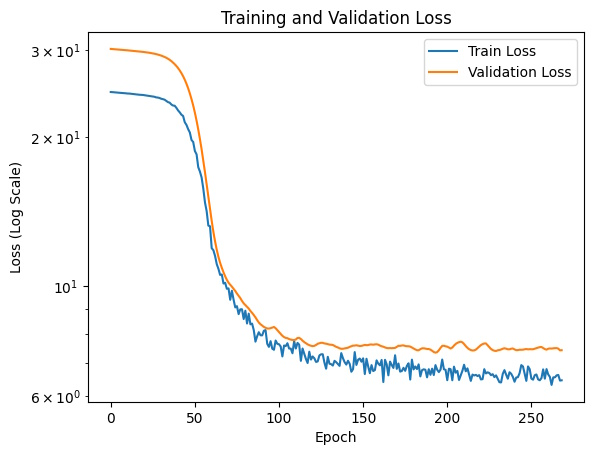
\includegraphics[width=0.45\textwidth]{images/autoencoder_loss.jpg}
    \caption{Training and validation loss of the autoencoder over epochs. The close alignment between the two curves indicates good generalization and absence of overfitting during training.}
    \label{fig:autoencoder-loss}
\end{figure}

\subsection{SVM Filtering of Synthetic Fraud Samples}
To improve the quality and realism of synthetic fraud data generated by the autoencoder, we introduced a filtering step using a Support Vector Machine (SVM). The goal of this step was to discard unrealistic or noisy synthetic examples that could degrade the training process of the subsequent classifier.

To train the SVM, a balanced dataset was constructed by randomly sampling an equal number of legitimate transactions to match the available genuine fraud samples. The two subsets were combined and assigned binary class labels, ensuring the SVM would learn a robust decision boundary between real fraud and legitimate data.

The combined dataset was shuffled and split into training and testing sets to evaluate generalization performance. A linear kernel was used for the SVM, prioritizing simplicity and interpretability. After training, the model achieved a training accuracy of \texttt{0.9438} and a testing accuracy of \texttt{0.9650}, indicating strong discriminative power on unseen samples.

Once trained, the SVM was applied to the synthetic samples generated by the autoencoder. Only those samples classified as fraudulent by the SVM were retained for the final training set. This filtering step significantly reduced the presence of unrealistic or misrepresentative samples, resulting in a cleaner, more trustworthy dataset for downstream classification.

After applying the SVM, only the synthetic samples classified as fraudulent were retained. This resulted in a final training set composed of \texttt{199008} legitimate and \texttt{199008} fraud samples, totalling \texttt{398016} samples used to train the ALSTM classifier.

\subsection{Attention-based LSTM Classifier}
To effectively detect fraudulent transactions in a sequential context, we employed an Attention-based Long Short-Term Memory (ALSTM) network as our final classification model. This choice is motivated by the observation that transaction sequences often contain temporal dependencies and behavioral patterns that are highly indicative of fraud.

\subsubsection{Motivation for Using ALSTM in Fraud Detection}
Fraudulent behavior frequently unfolds as a sequence of anomalies rather than isolated events. For example, fraudulent activity may be preceded by low-value "testing" transactions, rapid location changes, or abrupt deviations from typical purchasing behavior. Traditional feedforward networks lack the ability to capture these time-dependent patterns. ALSTM networks, by contrast, are well-suited for this task: the LSTM component models long-term dependencies across sequences, while the attention mechanism dynamically emphasizes the most relevant time steps for making predictions. This dual capability allows the model to prioritize significant contextual information during classification.

\subsubsection{Data Preparation and Input Format}
After generating a balanced dataset through synthetic fraud generation and SVM-based filtering, we reshaped the data to fit the expected input of the ALSTM network. Each sample was treated as a univariate sequence with a fixed length of 1 (since each transaction is an independent vector of features, not a true multistep temporal sequence).

\subsubsection{Model Architecture and Training}
The ALSTM architecture implemented in this project consists of the following components:
\begin{itemize}
    \item Two stacked LSTM layers, each with 50 hidden units, processing the transaction feature vectors. Both LSTM layers employed dropout regularization with a dropout rate of 0.3 and a recurrent dropout of 0.2 to prevent overfitting.
    \item A custom attention mechanism applied over the outputs of the second LSTM layer, dynamically weighting each time step's output to create a focused context vector.
    \item A fully connected dense layer receiving the attention-weighted context vector, producing the final output score.
\end{itemize}

The model was compiled using the Mean Squared Error (MSE) loss function. The \texttt{Adam} optimizer was chosen for its adaptive learning capabilities, with the initial learning rate set to $0.001$. The training process utilized early stopping and learning rate reduction upon plateauing validation loss to achieve robust convergence and avoid overfitting.

\subsection{Gradient Boosting Integration}
After training the Attention-based LSTM (ALSTM) model on the balanced dataset, we integrated it into a gradient boosting framework to further enhance predictive performance. The motivation behind this integration lies in the ability of gradient boosting to iteratively correct errors made by previous models, thereby improving overall classification accuracy—especially important in highly imbalanced scenarios like fraud detection.

In our approach, the ALSTM acts as a weak learner within the gradient boosting process. During each iteration, the boosting algorithm evaluates the residuals—i.e., the errors made by the current ensemble—and trains a new ALSTM model to minimize these errors. This is accomplished by computing the gradient of the loss function (binary cross-entropy) with respect to the model's predictions and using it to guide the training of subsequent learners.

To ensure stable and efficient convergence, we adopted a small learning rate for each boosting step and limited the number of boosting rounds to prevent overfitting. The final prediction is obtained by aggregating the outputs of all ALSTM learners, weighted according to their contribution in reducing the overall loss.